\documentclass[11pt]{article}
\usepackage{fullpage,amsmath,graphicx}

% --- -----------------------------------------------------------------
% --- Document-specific definitions.
% --- -----------------------------------------------------------------
\newtheorem{definition}{Definition}

\newcommand{\concat}{{\,\|\,}}
\newcommand{\bits}{\{0,1\}}

% --- -----------------------------------------------------------------
% --- The document starts here.
% --- -----------------------------------------------------------------
\begin{document}
\sloppy

\noindent Rutgers University\\
CS440: Introduction to Artificial Intelligence, Spring 2017\\
Kostas Bekris\\

\begin{center}
\LARGE{\textbf{Homework 4: James Carroll and Joel Carrillo}}\\
\large{\textbf{\emph{Decision Making under Uncertainty and Learning}}}
\end{center}

\vspace{.1in}

\begin{enumerate}

\item Question 1
\begin{enumerate}
\item Starting with an arbitrary discount of 0.4 and values (0, 0, 0, 0), it took one millisecond and five iterations to find the optimal policy of: Action 2 at State 1; Action 2 at State 2; Action 3 at State 3; and Action 1 at State 4. \\ \\
The optimal utility at the respective states are 0.14690304000000004, 0.39942144000000007, 1.1707264, and 0.43098624000000013. The method was repeatedly applying the Bellman equation to find the policy that maximizes the utility function. Intermediate values:
\begin{enumerate}
\item Policy [0, 0, 0, 0] Values [0, 0, 1, 0]
\item Policy [0, 0, 0, 0] Values [0, 0.32, 1, 0.36]
\item Policy [0, 1, 0, 0] Values [0.1152, 0.3456, 0.144, 0.3744]
\item Policy [1, 1, 2, 0]  Values [0.129024, 0.393728, 1.14976, 0.426816]
\item Policy [1, 1, 2, 0]  Values [0.14690304, 0.39942144, 1.1707264, 0.43098624]
\end{enumerate}
\end{enumerate}
\item Question 2
\begin{enumerate}
\item Yes.
\item Gain(GPA) = $I(\frac{p}{p+n}, \frac{n}{p+n})$ - Remainder(GPA) \\
$I(\frac{6}{6+6}, \frac{6}{6+6}) = I(\frac{1}{2}, \frac{1}{2}) = 1$ \\
Gain(GPA) = 1 - $\sum_{i=1}^{v} \frac{p_i + n_i}{p + n} I(\frac{p_i}{p_i + n_i},\frac{n_i}{p_i + n_i}) $ \\
Gain(GPA) = 1 - $[\frac{4}{12} I(0,1) + \frac{5}{12} I(\frac{3}{5}, \frac{2}{5}) + \frac{3}{12} I(1, 0)]$ \\
Gain(GPA) = 1 - $\frac{4}{12} * 0 + \frac{5}{12} * (0.9710) + \frac{3}{12} * 0 = 0.5954$ \\
Gain (Pub) = 1 - $[\frac{7}{12} I(\frac{3}{7}, \frac{4}{7}) + \frac{5}{12} I(\frac{3}{5}, \frac{2}{5}))] = 0.0207$ \\
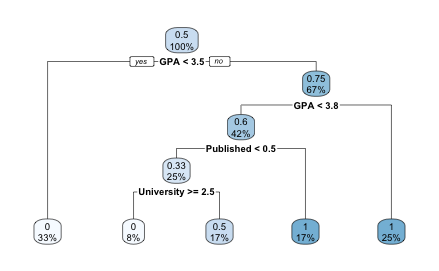
\includegraphics[scale=0.5]{gpaplot}
\item Yes, because the information gain for GPA is highest, Publications is second-highest, and so forth.
\end{enumerate}
\item Question 3
\begin {enumerate}
\item
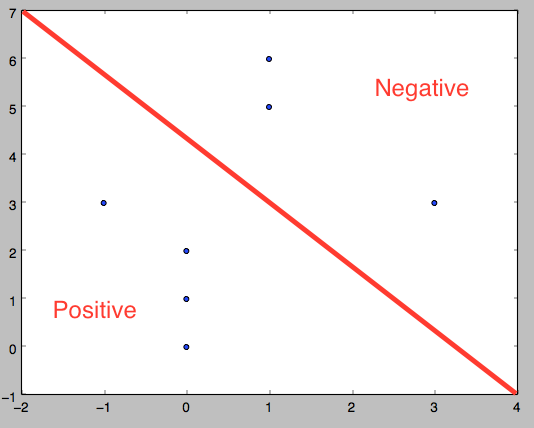
\includegraphics[scale=0.5]{svm}
\item For this line, w = ${-1.3164}$ and b = ${\text{4.2658}}$.
\item As the newly-added points do nothing to affect the separation of the training points overall, the linear SVM's values for w and b would remain the same.
\end {enumerate}
\item Question 4
\begin {enumerate}
\item
For the purposes of keeping the rest of the document clean, the coded printout is attached to the end of the document, after Question 5. This particular sample found the division in 14 total steps, but it can vary. \newline
The six lines prior depict the first six steps, including the initial line (step 0, in this case.) \newline
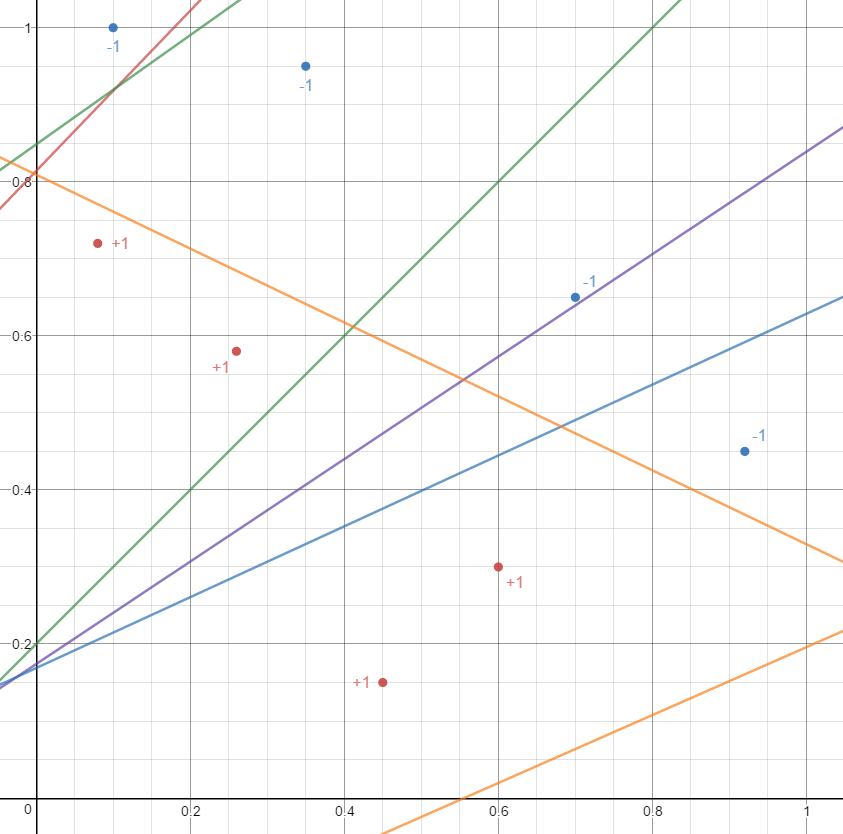
\includegraphics[scale=0.4]{graph1}
\item
This work is shown in (a), but the weights derived are the following: \newline
w0: 0.7 w1: -0.415 w2: -0.865
\item
Because the graph can only be depicted one-dimensionally, the best way to visualize this is a straight line along which all the samples' i$_{\text{1}}$ locations are placed. The minimum error is 2, with the two 'earliest' samples from Class -1 being cut off from the others. \newline
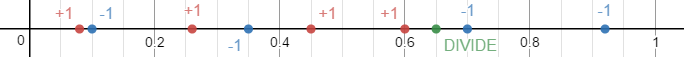
\includegraphics[scale=0.75]{graph2}
\end {enumerate}
\item Question 5
\begin {enumerate}
\item
The minimum error for this chart is 2, as shown below. It is impossible for a straight line to perfectly separate all the samples by the nature of the plotted samples. \newline
In the below chart, the value of the line is: -1.02098x + 0.97902, with weights w$_{\text{0}}$ = 0.7, w$_{\text{1}}$ = -0.730, w$_{\text{2}}$ = -0.715, where w$_{\text{0}}$ is the bias.
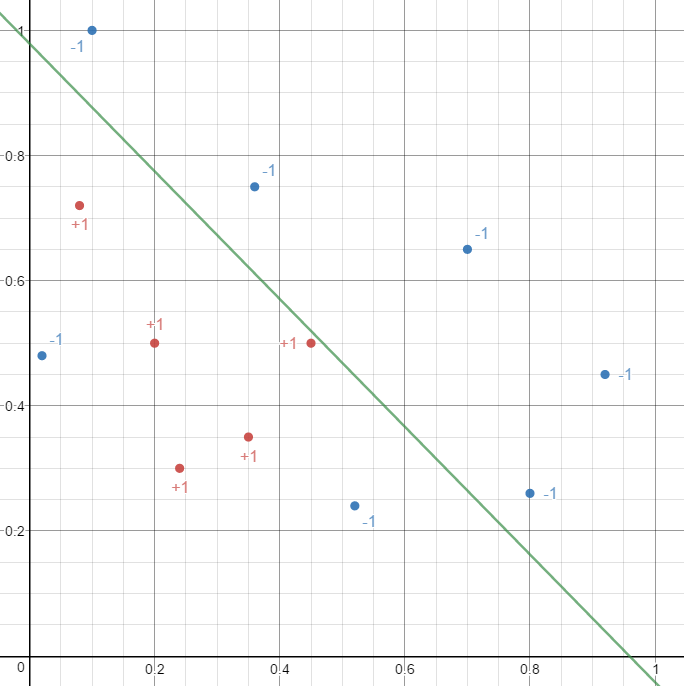
\includegraphics[scale=0.5]{graph3}
\item
In order to tackle this problem, we need to encapsulate the Class +1 samples in an area surrounded by Class -1 samples, effectively boxing it in. A multi-layer perceptron is required that should operate with the following steps:
\begin {enumerate}
\item Given input weights and a bias are inserted three times into three different 'hidden' perceptrons.
\item The hidden perceptrons calculate as normal, each with their own lines and their own means of determining missed specimens.
\item The perceptrons place their output in the 'output' perceptron, which uses these outputs as their own lines.
\item The output will check if the lines function as an 'area' and successfully encapsulate the Class +1 specimens, without allowing any Class -1 samples.
\item If it does, then stop. If not, then modify the weights inserted into each hidden perceptron until it is successful.
\end {enumerate}
We can actually use the unsuccessful line used in (a) towards this end. \newline 
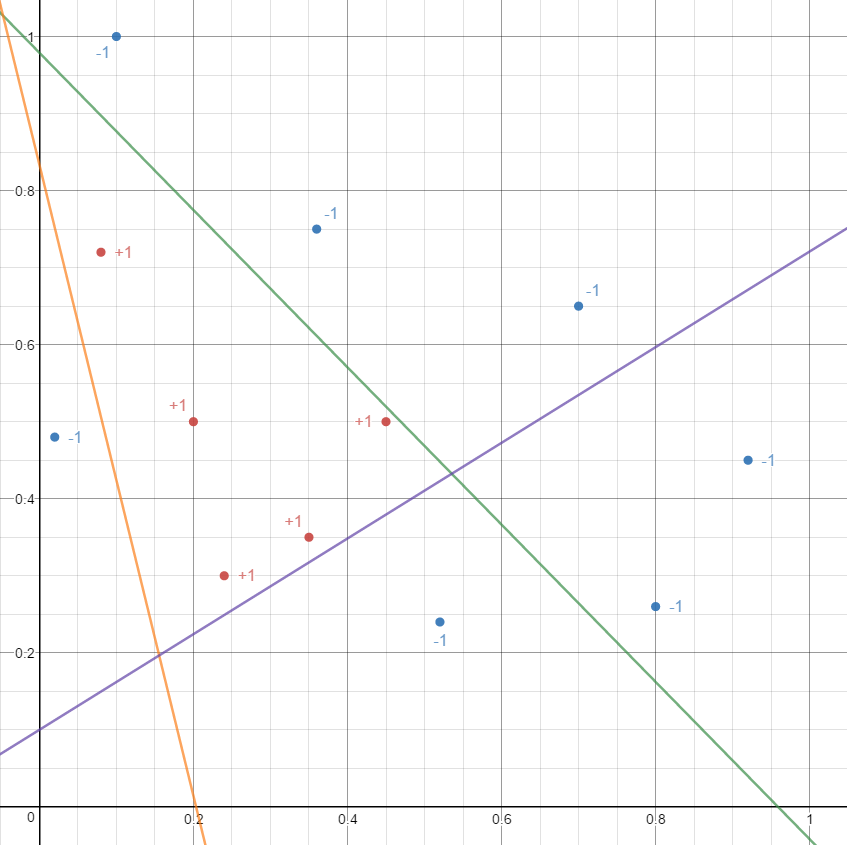
\includegraphics[scale=0.4]{graph4}
\item Line 1: -1.02098x + 0.97902 \newline Line 2: -4.09790x + .834 \newline Line 3: .62098x + 0.08379
\newline
\end {enumerate}
Question 4, Part (a) Code Printout: \newline
=================== \newline
step: 0 info: w0: 0.2 w1: 1.0 w2: -1.0 misses: 4 \newline
		slope: 1.0 bias/w2: -0.2 \newline
	visual line: 1.0x - -0.2 \newline
=================== \newline
step: 1 info: w0: -0.3 w1: 0.54 w2: -1.225 misses: 4 \newline
		slope: 0.44081632653061226 bias/w2: 0.24489795918367344 \newline
	visual line: 0.44081632653061226x - 0.24489795918367344 \newline
=================== \newline
step: 2 info: w0: 0.2 w1: 0.765 w2: -1.1500000000000001 misses: 3 \newline
		slope: 0.6652173913043478 bias/w2: -0.17391304347826086 \newline
	visual line: 0.6652173913043478x - -0.17391304347826086 \newline
=================== \newline
step: 3 info: w0: 0.7 w1: 0.895 w2: -0.8600000000000001 misses: 3 \newline
		slope: 1.0406976744186045 bias/w2: -0.8139534883720929 \newline
	visual line: 1.0406976744186045x - -0.8139534883720929 \newline
=================== \newline
step: 4 info: w0: 0.19999999999999996 w1: 0.545 w2: -1.185 misses: 3 \newline
		slope: 0.459915611814346 bias/w2: -0.16877637130801684 \newline
	visual line: 0.459915611814346x - -0.16877637130801684 \newline
=================== \newline
step: 5 info: w0: 0.7 w1: 0.5850000000000001 w2: -0.8250000000000001 misses: 3 \newline
		slope: 0.7090909090909091 bias/w2: -0.8484848484848484 \newline
	visual line: 0.7090909090909091x - -0.8484848484848484 \newline
=================== \newline
step: 6 info: w0: 0.19999999999999996 w1: 0.12500000000000006 w2: -1.05 misses: 3 \newline
		slope: 0.1190476190476191 bias/w2: -0.19047619047619044 \newline
	visual line: 0.1190476190476191x - -0.19047619047619044 \newline
=================== \newline
step: 7 info: w0: 0.7 w1: 0.25500000000000006 w2: -0.76 misses: 3 \newline
		slope: 0.3355263157894738 bias/w2: -0.9210526315789473 \newline
	visual line: 0.3355263157894738x - -0.9210526315789473 \newline
=================== \newline
step: 8 info: w0: 0.19999999999999996 w1: -0.09499999999999992 w2: -1.085 misses: 4 \newline
		slope: -0.08755760368663587 bias/w2: -0.184331797235023 \newline
	visual line: -0.08755760368663587x - -0.184331797235023 \newline
=================== \newline
step: 9 info: w0: 0.7 w1: -0.05499999999999992 w2: -0.725 misses: 2 \newline
		slope: -0.07586206896551713 bias/w2: -0.9655172413793103 \newline
	visual line: -0.07586206896551713x - -0.9655172413793103 \newline
=================== \newline
step: 10 info: w0: 0.19999999999999996 w1: -0.4049999999999999 w2: -1.05 misses: 4 \newline
		slope: -0.3857142857142856 bias/w2: -0.19047619047619044 \newline
	visual line: -0.3857142857142856x - -0.19047619047619044 \newline
=================== \newline
step: 11 info: w0: 0.7 w1: -0.10499999999999993 w2: -0.9 misses: 2 \newline
		slope: -0.11666666666666659 bias/w2: -0.7777777777777777 \newline
	visual line: -0.11666666666666659x - -0.7777777777777777 \newline
=================== \newline
step: 12 info: w0: 0.19999999999999996 w1: -0.4549999999999999 w2: -1.225 misses: 4 \newline
		slope: -0.37142857142857133 bias/w2: -0.16326530612244894 \newline
	visual line: -0.37142857142857133x - -0.16326530612244894 \newline
=================== \newline
step: 13 info: w0: 0.7 w1: -0.4149999999999999 w2: -0.8650000000000001 misses: 0 \newline
		slope: -0.4797687861271675 bias/w2: -0.8092485549132946 \newline
	visual line: -0.4797687861271675x - -0.8092485549132946 \newline
\end{enumerate}
\end{document}
